% !TEX root = ../00_thesis.tex

\section{System Model}
\label{sec:problem}

Let \flowset be the set of real-time message \emph{flows} in the system.
The message release of each flow is \emph{sporadic with jitter}; \ie each flow $\flowi = (\flowsrci,\flowdsti,\periodi,\jitteri,\deadlinei)$ is defined by a \emph{source application} running on \emph{source node} \flowsrci that \emph{releases} messages with a \emph{minimum message interval} \periodi and \emph{jitter} \jitteri ($\jitteri < \periodi$), such that the time span of $n$ successive messages is never smaller than $(n-1)\times\periodi - \jitteri$ for any $n$. Every message released at $n_i^s$ should be delivered to the application running on \emph{destination node} \flowdsti within the  same \emph{relative end-to-end deadline}~$\deadlinei$.


The system model is illustrated in \cref{fig:DRP_sysmodel}: a set of \emph{nodes}~\nodeset exchange messages over a wireless multi-hop network; messages sent from a source node to a destination node are possibly relayed by multiple other nodes.
A logically global network manager, called the \emph{host}, arbitrates access to the network. Physically, the host may be one of the nodes.
The source and destination applications of a flow \flowi run on physically distributed nodes \flowsrci and \flowdsti.
Nodes can send to and receive messages from all other nodes in the system.

\begin{figure}
  \centering
  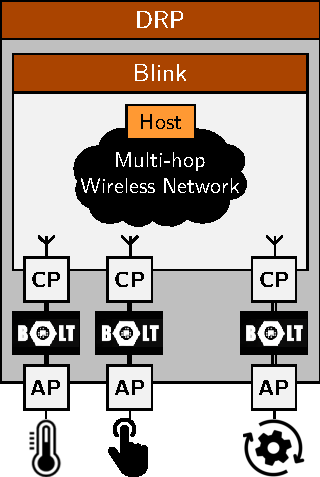
\includegraphics[scale=1]{stack_drp}
  \caption{System model of the \DRPLong (\DRP).
  \capt{A set~$\mathcal{N}$ of \DPP nodes are forming a wireless CPS.
  The communication processors (\CPs) run the \blink real-time protocol~\cite{zimmerling2017Blink} to exchange messages across a multi-hop wireless network.
  The \CPs forward and receive messages from their application processors (\APs) through \bolt~\cite{sutton2015Bolt}.
  \DRP is a global scheduler that arbitrates end-to-end communications between the \APs.
  On each \AP, the application tasks can be scheduled freely (\eg using a polling server, rate monotonic, \etc) as long as the resulting schedule satisfies the \DRP contracts~(\cref{sec:designDetailed}).
  The host is a (logically) global network manager which arbitrates the access to the shared wireless medium; \ie it runs the \blink and \DRP schedulers. Physically, one of the nodes plays the role of the host.}}
  \label{fig:DRP_sysmodel}
\end{figure}

\fakepar{Problem statement}
The problem is to design a wireless \CPS that fulfills all the requirements presented in \cref{sec:drp_intro} such that, for every message of every flow \flowi $\in \mathcal{F}$ released at the source node \flowsrci, if it is successfully transmitted by the wireless network, then it is delivered to the destination application running on node \flowdsti within the flow end-to-end deadline \deadlinei.

\squarepar{%}
  \fakepar{Application use case}
  Consider an acoustic wireless sensor network, such as those used to monitor permafrost in high alpine regions~\cite{weber2019decade,meyer2019IPSN}.
  Rock cracks are unpredictable events; however when one such event does happen, data must be collected and forwarded rapidly to a sink node for processing. For an early-warning system, it is crucial that this happens in real-time.
  Such an application perfectly matches our system model and motivates our problem statement.%
}
